\documentclass[a5paper]{article}
\usepackage[a5paper, top=8mm, bottom=8mm, left=8mm, right=8mm]{geometry}

\usepackage{polyglossia}
\setdefaultlanguage[babelshorthands=true]{russian}

\usepackage{fontspec}
\setmainfont{FreeSerif}
\newfontfamily{\russianfonttt}[Scale=0.7]{DejaVuSansMono}

\usepackage[font=scriptsize]{caption}

\usepackage{amsmath}
\usepackage{amssymb,amsfonts,textcomp}
\usepackage{xcolor}
\usepackage{array}
\usepackage{hhline}
\usepackage{cite}

\usepackage[hang,multiple]{footmisc}
\renewcommand{\footnotelayout}{\raggedright}

\PassOptionsToPackage{hyphens}{url}\usepackage[xetex,linktocpage=true,plainpages=false,pdfpagelabels=false]{hyperref}
\hypersetup{colorlinks=true, linkcolor=blue, citecolor=blue, filecolor=blue, urlcolor=blue, pdftitle=1, pdfauthor=, pdfsubject=, pdfkeywords=}

\usepackage{tabu}

\tabulinesep=1.2mm

\usepackage{graphicx}
\usepackage{indentfirst}
\usepackage{multirow}
\usepackage{subfig}
\usepackage{footnote}
\usepackage{minted}

\newcommand{\attribution}[1] {
\vspace{-5mm}\begin{flushright}\begin{scriptsize}\textcolor{gray}{\textcopyright\, #1}\end{scriptsize}\end{flushright}
}

\sloppy
\pagestyle{plain}

\title{Коллекции из стандартной библиотеки Java}
\author{Юрий Литвинов\\\small{yurii.litvinov@gmail.com}}

\date{30.01.2019}

\begin{document}

\maketitle
\thispagestyle{empty}

\section{Обзор библиотеки}

В Java есть довольно развитая библиотека коллекций (ну, как и в любом языке), и, как и в любом языке, в ней есть свои особенности и архитектурные изыски. В Java библиотека проектировалась исходя из требований минимальности и простоты интерфейсов коллекций, единообразия и простоты расширения сторонними разработчиками. Посмотрим, что получилось.

Библиотека состоит из следующих основных частей.

\begin{itemize}
	\item Интерфейсы коллекций --- описывают контракты, которые должны выполнять реализации, типа списка, отображения, множества. Любая библиотечная коллекция реализует один или несколько этих интерфейсов, и чтобы самописные коллекции работали с библиотечными алгоритмами нормально, они тоже должны эти интерфейсы реализовывать. Рекомендуется в коде использовать коллекции именно по их интерфейсам.
	\item Реализации общего назначения --- стандартные реализации, которые рекомендуется использовать в большинстве случаев.
	\item Специализированные реализации --- реализации, нужные для разных необычных случаев (например, EnumSet и EnumMap, заточенные под хранение элементов enum-ов).
	\item Многопоточные реализации, про которые мы, надеюсь, поговорим, когда дойдём до многопоточности.
	\item Абстрактные реализации --- нужны для удобного создания своих коллекций, соответствующих всем правилам стандартной библиотеки. С их помощью можно быстро сделать, например, список, хеш-таблицу и всё такое, реализовав пару обязательных методов, а все остальные методы абстрактная реализация предоставит сама, на основе пары реализованных. При желании можно переопределить и любой другой метод так, чтобы он реализовывал свою функциональность более эффективно.
	\item Обёртки позволяют взять коллекцию и наделить её каким-нибудь свойством, например, взять список и сделать его немутабельным. Или потокобезопасным.
	\item Алгоритмы работают над стандартными коллекциями и делают всякие полезные вещи: сортировку, поиск минимума-максимума, копирование и т.д.
	\item Инфраструктура --- это различные штуки, используемые в интерфейсах коллекций, такие как итераторы, компараторы, исключения и т.д.
\end{itemize}

\section{Основные интерфейсы}

Интерфейсы коллекций --- пожалуй, самое важное в библиотеке, потому что они определяют всю её архитектуру. Вот самые основные:

\begin{itemize}
	\item Iterable --- всё, по чему можно итерироваться. 
	\item Collection --- просто группа объектов. Вводит понятие ``размер коллекции'' (Iterable может быть бесконечным) и операции добавления, удаления, проверки на принадлежность.
	\begin{itemize}
		\item Set, SortedSet --- множества. Не допускают повторяющихся элементов. SortedSet содержит элементы в натуральном порядке или в порядке, определённом компаратором --- и имеет дополнительные методы, использующие тот факт, что элементы упорядочены (например, найти самый большой элемент).
		\item List --- упорядоченная коллекция, вводит понятие ``позиция'' и возможность управлять конкретным положением элемента в списке. Обратите внимание, что, поскольку в Java нет перегрузки операторов, доступ к элементу по заданной позиции выполняется методом --- at(). Обход списка выгоднее выполнять итератором.
		\item Queue, Deque --- очереди, деки. Интересно, что у очередей есть два сорта операций для выполнения одного и того же действия --- те, которые бросают исключение, если что-то не так, и те, которые возвращают специальное значение. Например, remove() и poll().
	\end{itemize}
	\item Map --- отображение. Коллекцией не является, но позволяет получить коллекции ключей, значений и пар ``ключ-значение''.
	\begin{itemize}
		\item SortedMap --- отображение, где ключи упорядочены (опять-таки, в натуральном порядке или в порядке, задаваемом компаратором). Упорядоченность ключей проявляется при обходе коллекций ключей и пар ``ключ-значение''.
		\item NavigableMap --- SortedMap, который ещё позволяет получить элемент, ближайший к искомому (например, найти наибольший элемент, меньший данного).
	\end{itemize}
\end{itemize}

\section{Реализации}

Основные реализации библиотечных интерфейсов приведены в таблице ниже. Как обычно, есть выбор, использовать массивы или указатели как внутреннее представление данных для списков, и деревья либо хеш-таблицы для отображений и множеств. Более экзотические реализации --- это LinkedHashSet и LinkedHashMap, они используют ``провязанную'' хеш-таблицу. То есть всё работает как обычная хеш-таблица, но ещё и можно итерироваться по элементам в порядке их добавления.

\begin{footnotesize}
	\begin{tabu} {| X[1 l p] | X[0.7 l p] | X[1 l p] | X[0.7 l p] | X[1 l p] | X[1.3 l p] |}
		\tabucline-
		Интерфейс  & Хеш-таблица  & Массив      & Дерево   & Список      & Хеш-таблица + Список  \\
		\tabucline-
		\everyrow{\tabucline-}
		Set        & HashSet      &             & TreeSet  &             & LinkedHashSet         \\
		List       &              & ArrayList   &          & LinkedList  &                       \\
		Deque      &              & ArrayDeque  &          & LinkedList  &                       \\
		Map        & HashMap      &             & TreeMap  &             & LinkedHashMap         \\
	\end{tabu}
\end{footnotesize}

Реализации из этой таблицы предназначены для использования в самом общем случае, и в своих программах следует стараться пользоваться именно ими. Однако, есть несколько специализированных реализаций и развитая инфраструктура для встраивания своих реализаций в библиотеку. Её мы будем использовать очень часто, потому что типичное условие домашки или контрольной до конца модуля будет выглядеть как ``реализуйте какую-нибудь неведомую структуру данных так, чтобы она предоставляла такие-то стандартные интерфейсы''.

Для реализации своих коллекций в библиотеке есть классы AbstractCollection, AbstractSet, AbstractList, AbstractSequentialList, AbstractMap. Предполагается, что если вы хотите реализовать свою коллекцию, вы наследуетесь от этих классов, реализуете некоторые важные методы, а остальные методы, реализованные в абстрактных классах, будут просто использовать ваши реализации, так что вам не надо будет о них думать. Если производительность не важна, как правило, пары-тройки методов достаточно для того, чтобы коллекция работала. Например, AbstractCollection используется для того, чтобы реализовать просто какую-то коллекцию так, чтобы она предоставляла интерфейс Collection. Можно было бы реализовать интерфейс Collection и вручную, но у него что-то около 20 методов, некоторые ваши предшественники на контрольной пытались, не не успели. Наследуетесь от AbstractCollection, переопределяете метод iterator() так, чтобы он возвращал Iterator, умеющий делать hasNext() и next() с вашей коллекцией. Ещё надо переопределить size(). Если вы хотите немутабельную коллекцию, то этого достаточно, иначе надо ещё переопределить add() и remove() для итератора (да, remove() не в самой коллекции, а в итераторе, с ней связанном). Кроме того, по соглашению должно быть два конструктора --- один без аргументов (создающий пустую коллекцию), второй --- принимающий Collection (и создающий её копию). Остальные методы определены в AbstractCollection так, чтобы использовать эти базовые (например, addAll() будет просто вызывать ваш add() для каждого элемента). Естественно, реализации по умолчанию вас могут не устраивать с точки зрения производительности, так что их можно (и иногда нужно) переопределить.

AbstractMap --- несколько более сложный пример. Чтобы сделать своё отображение, достаточно реализовать метод entrySet(), который возвращает так называемый ``View Set'' из объектов \mintinline{java}|Map.Entry<K,V>|, который должен содержать все пары из отображения, причём сам он элементы не хранит, а просто предоставляет доступ к элементам своего отображения в виде множества. Обычно этот View Set сам реализуется на базе AbstractSet. Чтобы отображение было мутабельным, надо ему переопределить метод put() и remove() для итератора, возвращаемого entrySet().iterator(). Ну и нетрудно догадаться, как реализованы методы в AbstractMap --- мы просто берём итератор и перебираем пары, пока не найдём нужную. Поскольку вам отображение, работающее за линейное время, скорее всего, не нужно, тут наверняка придётся ключевые методы переопределить.

\section{Инфраструктура}

Ключевые интерфейсы, необходимые для сопровожения коллекций, во-первых, включают в себя Iterator (и интерфейс Iterable, который декларирует возможность вернуть итератор). Итератор вообще --- это один из паттернов проектирования, отделяющий логику обхода коллекции от её внутреннего представления, по сути, обёрнутая в объект ссылка на текущий элемент коллекции плюс способ получить следующий. Java-style-итераторы несколько отличаются от C++-ных и C\#-овских, тем, что они возвращают элемент только когда мы переходим на следующий. Методы у Java-style-итераторов такие:

\begin{itemize}
	\item hasNext() возвращает true, если есть следующий элемент;
	\item next() возвращает сам следующий элемент и продвигает итератор;
	\item remove() удаляет из коллекции текущий элемент. Метод опциональный, его можно не реализовывать, а бросать UnsupportedOperationException. Но если реализовали, remove() должно быть можно вызывать только один раз на каждый вызов next().
\end{itemize}

Итераторы обычно реализуются как private вложенные классы в коллекции, коллекция возвращает итератор по интерфейсу Iterator. Итераторы ещё должны следить за своей коллекцией и бросать ConcurrentModificationException, если коллекция изменилась в процессе обхода, если коллекция явно не разрешает так делать и если это изменение --- не вызов remove самого итератора.

Ещё бывает ListIterator, для итерирования конкретно по спискам --- он двунаправленный и знает про индексы элементов.

Кроме итератора, важная штука --- это компаратор (интерфейс Comparator). Он позволяет установить отношение порядка над элементами. Интерфейс декларирует всего один метод, compare, возвращающий -1, 0 или 1 и обязанный подчиняться традиционным правилам полного порядка (транзитивность, антисимметричность и т.д.). Есть ещё интерфейс Comparable --- он внезапно не декларирует возможность объекта возвращать компаратор, а наоборот, задаёт альтернативный компаратору способ сравнения --- Natural Ordering. Интерфейс декларирует метод compareTo, который должен обладать свойствами, аналогичными compare() у компаратора, и если компаратора нет, все коллекции, которым нужен порядок элементов, используют compareTo. Собственно, порядок, задаваемый методом compareTo, и называется натуральным порядком. Натуральный порядок для какого-либо класса может быть только один, а вот компараторов может быть много разных.

Вот диаграмма, показывающая взаимосвязь основных коллекций, итераторов и их реализаций по состоянию на Java 1.4. Java 1.4 давным-давно в прошом, но существенных изменений в стандартных коллекциях не было, так что по большей части картинка из чрезвычайно годной книжки Брюса Эккеля ``Thinking in Java'' всё ещё актуальна:

\begin{center}
	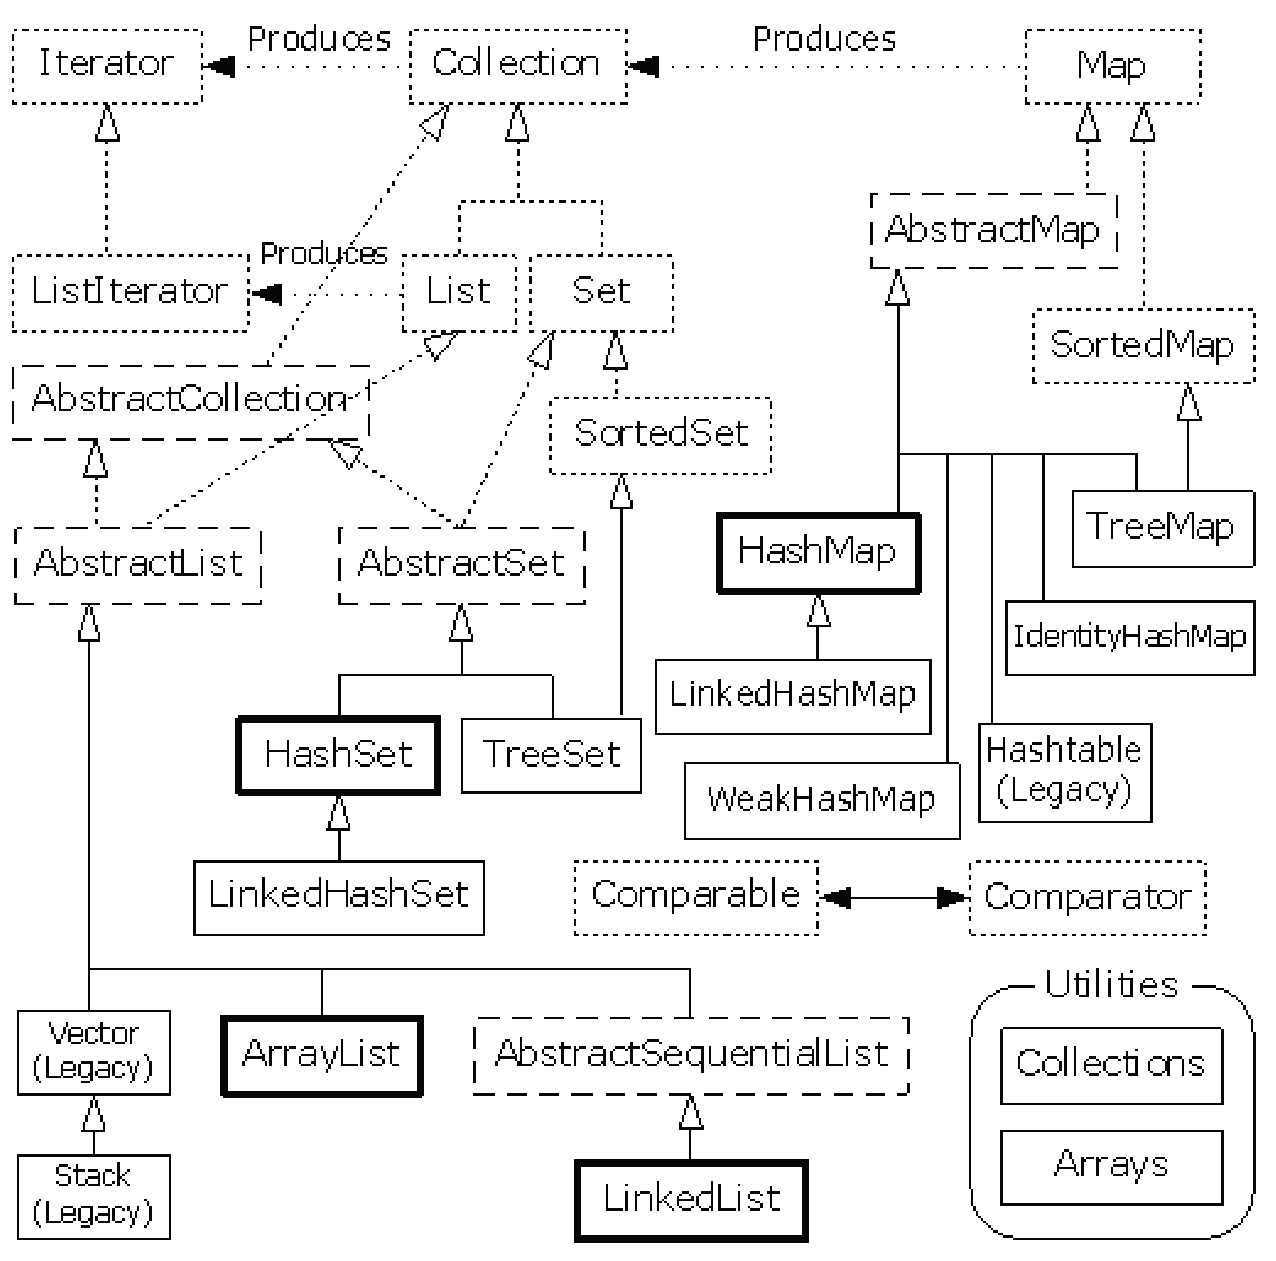
\includegraphics[width=0.6\textwidth]{java4Containers.png}
	\attribution{B. Eckel, Thinking in Java}
\end{center}

\section{Исключения}

Основные исключения, которые бросает подсистема коллекций:

\begin{itemize}
	\item UnsupportedOperationException --- реализация не поддерживает метод, объявленный в интерфейсе (в документации такой метод должен быть помечен как optional);
	\item ConcurrentModificationException --- попытка продолжить обход итератором изменившейся коллекции если эта коллекция не позволяет это сделать и если мы не модифицировали коллекцию самим же итератором;
	\item NullPointerException, когда мы пытаемся что-то сделать с null-ами и коллекция этого не позволяет;
	\item ClassCastException, когда мы пытаемся делать с коллекцией что-то, что огорчает систему типов (например, попытка добавить в TreeMap что-то, что не умеет сравнивать компаратор);
	\item IndexOutOfBoundsException, когда мы обращаемся по индексу к элементу списка, но такого индекса в списке нет;
	\item NoSuchElementException, когда итератор дошёл до конца коллекции и мы всё равно пытаемся сделать next().
\end{itemize}

\section{Утилиты}

Помимо собственно коллекций есть статические классы, которые делают работу с коллекциями значительно более приятной. Во-первых, это класс java.util.Collections, содержащий в себе разные интересные методы, работающие для любых коллекций. Во-первых, это методы, типичные для подобного рода библиотек: binarySearch (искать в отсортированной коллекции, за log(n), если коллекция поддерживает интерфейс RandomAccess), copy, sort, shuffle (перемешать элементы коллекции, внезапно весьма удобный метод) и т.д. Ещё есть методы-фабрики: emptyList, emptyMap и т.д., создающие пустые немутабельные соответствующие коллекции; singleton, singletonList и т.д., создающие немутабельные коллекции, содержащие только один (указанный параметром) объект. И методы, создающие коллекции-обёртки: unmodifiableList, unmodifiableMap и т.д. Они принимают обычную коллекцию, а возвращают коллекцию, которую невозможно изменить через её методы (например, add будет бросать UnsupportedOperationException). На самом деле, возвращённая коллекция --- это \textit{вид} на оригинал, так что изменения исходной коллекции будут видны и в её немодифицируемом варианте.

Ещё есть утилиты для работы с массивами: java.util.Arrays. Там тоже имеются разные полезные методы, типа sort, compare, equals, fill и т.д., причём для разных примитивных типов. Чтобы с массивами было удобно работать как с коллекциями, есть метод Arrays.asList, представляющий массив в виде списка (тоже на самом деле это вид на массив, так что они остаются связаны).

\end{document}
